

\section{Solving linear inequalities }

In the United States temperatures for everyday things like the weather or cooking are given in Fahrenheit, denoted $^\circ$F.  In this system, water freezes into ice at $32^\circ$F and boils into steam at $212^\circ$F.  A common setting for room temperature is $68^\circ$F whereas average human body temperature is around $98.6^\circ$F.  And, most importantly, chocolate brownies bake at $350^\circ$F.

In the sciences, medicine, and most other countries, temperatures are measured in Celsius, denoted $^\circ$C.  (For those of us who grew up in the 1960s or earlier, ``Celsius'' is the temperature scale formerly known as ``centigrade.'') 
For comparison's sake, it's useful to know that water freezes at $0^\circ$C and boils at $100^\circ$C.  Not coincidentally -- it was set up that way.  Room temperature is $20^\circ$C whereas now average human body temperature is $37^\circ$C.  And those brownies? 
 
A common conversion is given by the equation $$F = 1.8C+32$$ 
where 
\begin{center}
\begin{tabular} {l} 
$F=$ Fahrenheit temperature ($^\circ$F) $\sim$ dep \\
$C=$ Celsius temperature ($^\circ$C) $\sim$ indep \\ 
\end{tabular}
\end{center}
You may have seen this equation before with fractions in it:  $F = \frac{9}{5}C + 32$.  Just another way to write the equation, since $\frac{9}{5} = 9 \div 5 = 1.8$.  
For example, when $C=100$ we have $$F= 1.8 \ast 100 + 32 =1.8 \times \underline{100}+32= 212 \quad \checkmark$$   You can (and should check) the other examples in our story.
 
 What about those chocolate brownies?  
We are looking for $F=350$.  That's the dependent variable, so you can practice your  linear equation solving skills to find the independent variable, $C$.  It turns out that chocolate brownies bake at around $177^\circ C$.

But, actually, chocolate brownies just need to bake in a ``moderate oven,'' which means between $325^\circ F$ and $375^\circ F$.  Let's first figure out when the oven temperature is under $375^\circ F$.  We want to know when $$F \le 375$$
so we have an inequality instead of an equation. Remember $\le$ stands for \textbf{less than or equal to}. Using  $F=1.8C+32$ we get $$1.8C+32 \le 375$$  We're looking for values of $C$ that make the left-hand side a number that's smaller than, or maybe as large as, 375, but no larger.  Quick vocabulary.  Equations have equal signs (=).  When we have inequality signs ($\le$, $\ge$, $>$, or $<$), it's called an \textbf{inequality} instead.

To solve this inequality we begin the same way as we would if we were solving the equation, by subtracting 32 from each side to get
 \begin{eqnarray*}
1.8C + \cancel{32}& \le &375  \\
-\cancel{32}& & -32  \\
\end{eqnarray*}
which simplifes to $$1.8C\le375-32=343$$  
% 325 is 162.777777... \approx 163

To understand why the inequality stays the same when we subtract the same number from both sides, think of the inequality as \begin{center} ``little'' $\le$ ``big'' \end{center}  If one number is littler than the other, the same will be true when we take away equal amounts.  So, for example, say that you have more cash than I do and we each buy a \$12 movie ticket -- maybe you have \$21 to start with but I only have \$18.  Afterwards, it will still be true that you have more cash than I do. You will have \$21 - \$12 = \$9 left but I will only have \$18 - \$12 = \$6.  I mean, we each will have less cash than before we bought the ticket, but you still have more than I do.  Which is why you should buy the popcorn.  But I digress.  % JODY -- I think something is needed here but these stories are too corny.  (Ha! popcorn, corny.)

Back to our example.  We had  $1.8C\le343$. Divide each side by 1.8 to get
$$\frac{\cancel{1.8}C}{\cancel{1.8} }\le \frac{293}{1.8}$$
which simplifies to $$C\le \frac{293}{1.8}= 293 \div 1.8 = 190.555555\ldots \approx 190^\circ C$$
The oven should be set at most $190^\circ C$.  We rounded down because we do not want the brownies to burn.

To understand why the inequality stays the same when we divided each side by the same number, think again of the inequality as \begin{center} ``little'' $\le$ ``big'' \end{center}  If one number is littler than the other, the same will be true when we divide both amounts by the same number.  So, for example, suppose we decided against buying popcorn so that  that you have \$9 left from the movie and I only had \$6. While we're making up stories, suppose we each have three children, who bought their own tickets but want some money from us for treats.  We each divide our remaining cash among our three children, respectively.  Yours each get $\$9\div 3 = \$3$ but mine only get $\$6\div3 =\$2$.  So mine get less than yours.

There is a little bit of caution when solving inequalities.  When symbolically solving an equation, any operation you do to both sides preserves the equality -- start with equal amounts, do same thing to each, end with equal amounts.  But, when symbolically solving an  inequality, only some operations you do to both sides preserve the inequality -- add or subtract from both sides, multiply or divide both sides by the same (positive) number.  But other operations can reverse the inequality.  

For example, we can swap sides of an equation, but if we swap sides of an inequality then the direction of the sign reverses.  In this brownie example, we want $$F \ge 325$$ Remember $\ge$ stands for \textbf{greater than or equal to}.  We can rewrite that inequality as $$325 \le F$$  In each case, $325$ is ``little'' and $F$ is ``big''.  Make sense?  Multiplying or dividing by a negative number switches the inequality sign as well.  Watch out for that with decreasing functions because that's where the slope is negative.  And we're dividing by the slope. % SU was "slope" used in 2.1?

Remember that the recipe for chocolate brownies says to bake in a moderate oven, between $325^\circ F$ and $375^\circ F$.   We just figured out that $F \le 375$ corresponds to $C \le 190$.  But that's only half of the story.  We also wanted $F \ge 325$.  While we could solve that inequality separately, it turns out there's an easier way.
Inequalities are a very useful notation for indicating ``between''.  We want between $325^\circ F$ and $325^\circ F$ to bake the brownies.  We can write $$325 \le F \le 375$$  
which is read \begin{center} ``$F$ is between 325 and 375 (inclusive)'' \end{center}  The word \textbf{inclusive} indicates that we're allowing $F=325$ or $F=375$. 

The good news is that we can solve this chain of inequalities all at once using the same steps as before but now being sure to do the same thing to all \emph{three} sides.  ``\emph{Three} sides?'' you ask.  Yes, ``three,'' I confirm.  Watch how this works. 
Start with$$325 \le F \le 375$$ Using $F=1.8C + 32$ we get $$325 \le 1.8C + 32 \le 375$$  Subtract 32 from each of the three sides to get
\begin{center}
\begin{tabular} {ccc cc}
325 & $\le$ & 1.8C + \cancel{32} &  $\le$ & 375 \\ 
-32 && \hspace{.45in}-\cancel{32} && -32 \\  %HSPACE
\end{tabular}
\end{center}
\noindent which simplifies to $$293 \le 1.8C \le 343$$

Next, divide all three sides by 1.8 to get
\begin{center}
\begin{tabular} {ccc cc}
$\frac{293}{1.8}$ & $\le$ &$\frac{\cancel{1.8}C}{\cancel{1.8}}$ &  $\le$ & $\frac{343}{1.8}$ \\
\end{tabular}
\end{center}
\noindent which simplifies to $$293\div 1.8 \le C \le 343 \div 1.8$$ so, $$ 162.777777... \le C \le 190.555555...$$
Best yet, say $$163 \le C \le 190$$  Chocolate brownies bake between $163^\circ C$ and $190^\circ C$.  Oven actually aren't that precise, so somewhere between $170^\circ C$ and $190^\circ C$ should do the job.

See the highlighted region in the graph?  That's the range of temperatures corresponding to $325-375^\circ$F or, as we have now discovered, $163-190^\circ$C.
\begin{center}
\scalebox {.8} {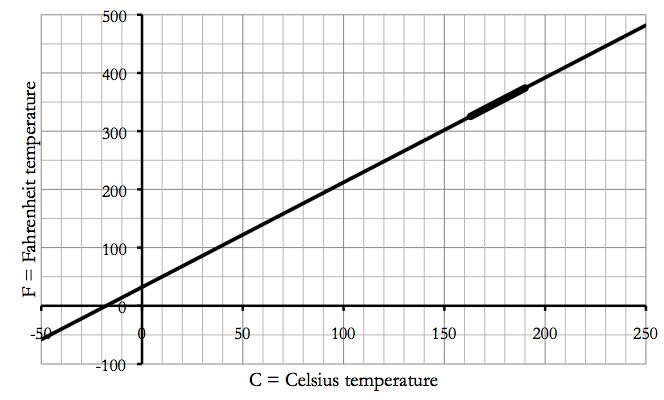
\includegraphics [width = 6in] {fahrenheitcelsius.png}}
\end{center}


%\newpage

%%\section{Solving linear inequalities}

 \begin{center}
\line(1,0){300} %\line(1,0){250}
\end{center}

\section*{Homework}

\noindent \textbf{Start by doing Practice exercises \#1-4 in the workbook.}

\bigskip

\noindent \textbf{Do you know \ldots}

\begin{itemize}
\item Common phrases that indicate an inequality? 
\item How to represent the idea of ``between'' using a double-sided inequality? 
\item Why we ``do the same thing to each side'' of an inequality when solving? 
\item How to solve a linear inequality? A chain of inequalities?
\item Why the inequality sign is reversed if we switch sides of the equation? 
\item When to solve an inequality, as opposed to solving an equation? 
 \item[~] \textbf{If you're not sure, work the rest of exercises and then return to these questions.  Or, ask your instructor or a classmate for help.}
\end{itemize}

\subsection*{Exercises}

\begin{enumerate} 
\setcounter{enumi}{4}

\item  Recall that the conversion between Fahrenheit ($F$) and Celsius ($C$) temperatures is given by the equation $$F = 1.8C+32$$
\begin{enumerate}
\item Evaluate the equation at the appropriate values to check that $0^\circ$C$=32^\circ$F, $20^\circ$C$=68^\circ$F, and $37^\circ$C$=98.6^\circ$F.
\item Set up and solve an equation to find the Celsius equivalent of brownie-baking temperature ($350^\circ$F).
\item You're planning a trip to Norway over Christmas and have heard it's will be around 10$^\circ$C.  What sort of jacket will you need?  Convert to Fahrenheit to decide. 
\item You want to explain to your Norwegian hosts that back in Minnesota this time of year temperatures can range between -20$^\circ$F and 40$^\circ$F.  Express this range in Celsius instead.  Set up and solve a chain of inequalities.
\item Your Norwegian hosts ask about the temperature in Minnesota during the summer.  You explain that summer temperatures typically range from 55$^\circ$F and 105$^\circ$F.  Express this range in Celsius instead.   Set up and solve a chain of inequalities.
\end{enumerate}

\item After borrowing some money through a line of credit on my bank account, I started paying off the interest plus \$250 a month.  Even once the loan is paid off I plan to continue to deposit \$250 each month to start savins.  That means my balance is given by the equation
$$A = 250M- \text{2,189.57}$$
where $M$ is the number of months since the loan and $A$ is the account balance, in dollars. \hfill \emph{Story also appears in 2.1 \#3}
\begin{enumerate}
\item Set up and solve an inequality to determine when I will have paid off my line of credit. That means the account balance will be \$0 or more.
\item Set up and solve an inequality to determine when I will have saved at least \$2,000.
\end{enumerate}  

\item When Gretchen walks on her treadmill, the number of calories per mile that she burns is given by the equation $$C=125M$$ where $C$ is the number of calories Gretchen burns by walking $M$ miles.  

\hfill \emph{Story also appears in 2.1 and 3.1 Exercises}
\begin{enumerate}
\item Draw a graph showing the number of calories Gretchen burns if she walks 0, 1, 2, or 3 miles.
\item How far does she need to walk to burn at least 200 calories? Set up and solve an inequality.
\item Highlight the part of your graph where she burns at least 200 calories.
\end{enumerate}

\item The water in the local reservoir has been dropping steadily.  In fact, $$D = 47-1.5W$$ where $D$ is the depth of the water (in feet) after $W$ weeks.  Any depth below 20 feet is considered dangerously low.  When will that happen, assuming no change in the weather?  Set up and solve an inequality.  And, check your answer.

\hfill \emph{Story also appears in 2.1 \#2 and 4.1 \#3}

\item A manufacturer makes family-sized bags of potato chips, advertised as containing 200 grams each.  In fact it's difficult to control the exact weight of a bag of potato chips, so it varies. The standard deviation is rather high, about 3.8 grams per bag.  The company would rather have bags too heavy than too light, lest they be accused of false advertising, so their average bag actually weighs 207 grams.  It turns out that approximately 97\% of all bags of chips weigh 200 grams or more.  We can compute the standard $Z$-score of a given bag of chips weighing $B$ grams using the equation $$Z = \frac{B-207}{3.8}$$
\begin{enumerate}
\item What is the $Z$-score for a bag of potato chips weighing the advertised 200 grams?  Remember above average $Z$-scores are positive and below average $Z$-scores are negative, so your answer should be negative.  
\item About \nicefrac{3}{4} of all bags of chips will have $Z \ge -.67$.  What weight bag has $Z$-score of $-.67$?  Set up and solve an inequality.
\item A standard $Z$-score between -1 and +1 is considered ordinary.  What weight bags are considered ordinary? 
\item Oh, and if a serving size is 28 grams (approximately 1 ounce), how many servings are in a bag that weights 207 grams?
\end{enumerate}

\item  The cost of vacation to Cork, Ireland from the Minneapolis/St. Paul airport for two people is given by the equation formula $$C = \text{2,828} + 310N$$ where $C$ is the total cost in U.S. dollars and $N$ is the number of days.  Ciara wants to take her boyfriend Seamus to Cork to meet Ciara's grandmother.
\begin{enumerate}
\item What would it cost Ciara to go to Ireland with Seamus for six days?
\item What might the number \text{2,828} mean in terms of the story, and what are its units?
\item What might the number 310 mean in terms of the story, and what are its units?
\item  If Ciara has budgeted up to \$\text{10,000}, how many days can they afford to spend in Ireland? Set up and solve an inequality to find the answer.
\end{enumerate}

\end{enumerate}


